\section{Introducción}

\begin{frame}{Introducción}

\begin{block}{Sistemas de videovigilancia automatizados}
\justifying
Han despertado un gran interés en los últimos años en la monitorización de lugares públicos y privados.
\vspace{0.2cm}
\end{block}

\begin{itemize}
    \justifying
    \item En los últimos tiempos la detección de objetos abandonados se ha investigado para detectar eventos de gran interés como \textbf{objetos abandonados} y \textbf{vehículos estacionados} ilegalmente.
    \item Los desarrollos de técnicas de detección de objetos abandonados se encuentran constantemente enfrentados contra diferentes \textbf{desafíos} durante su implementación.
    \item Los sistemas de detección de objetos abandonados actuales se centran principalmente en dos etapas principales: \textbf{detección estacionaria} y \textbf{clasificación de objetos}.
\end{itemize}

\end{frame}

%%%%%%%%%%%%%%%%%%%%%%%%%%%%%%%%%%%%%%%%%%%%%%%%%%%%%%%%%%%%%%%%%

\begin{frame}{Introducción}

\justifying
Los objetos abandonados se pueden determinar mediante dos reglas: el objeto aspirante se encuentra estático o desatendido.

\vspace{0.1cm}

\begin{itemize}
    \justifying
    \item El primer enfoque corresponde a una regla espacial, en la que un objeto se considera desatendido si el propietario del objeto se encuentra apartado del objeto.
    
\end{itemize}
    
\vspace{0.3cm}

\begin{figure}[ht]
\centering
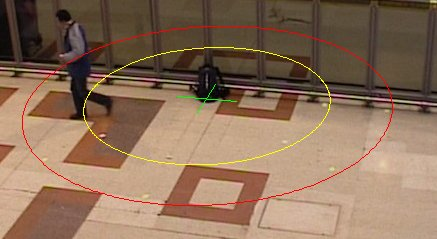
\includegraphics[width=0.4\textwidth]{Images/introduccion/pets2006-3m.jpeg}
\caption{\label{fig:pets2006-3m}Persona sobrepasando la zona de alarma (marcado en amarillo)}
\end{figure}
    
\end{frame}

%%%%%%%%%%%%%%%%%%%%%%%%%%%%%%%%%%%%%%%%%%%%%%%%%%%%%%%%%%%%%%%%%

\begin{frame}{Introducción}

\begin{itemize}
    \justifying
    \item El segundo enfoque define una regla temporal en la que un objeto se considera estacionario si se encuentra inmóvil durante un cierto período de tiempo, dependiendo de la aplicación, siendo típicamente 30 o 60 segundos.
    
\end{itemize}
    
\vspace{0.3cm}

\begin{figure}[ht]
\centering
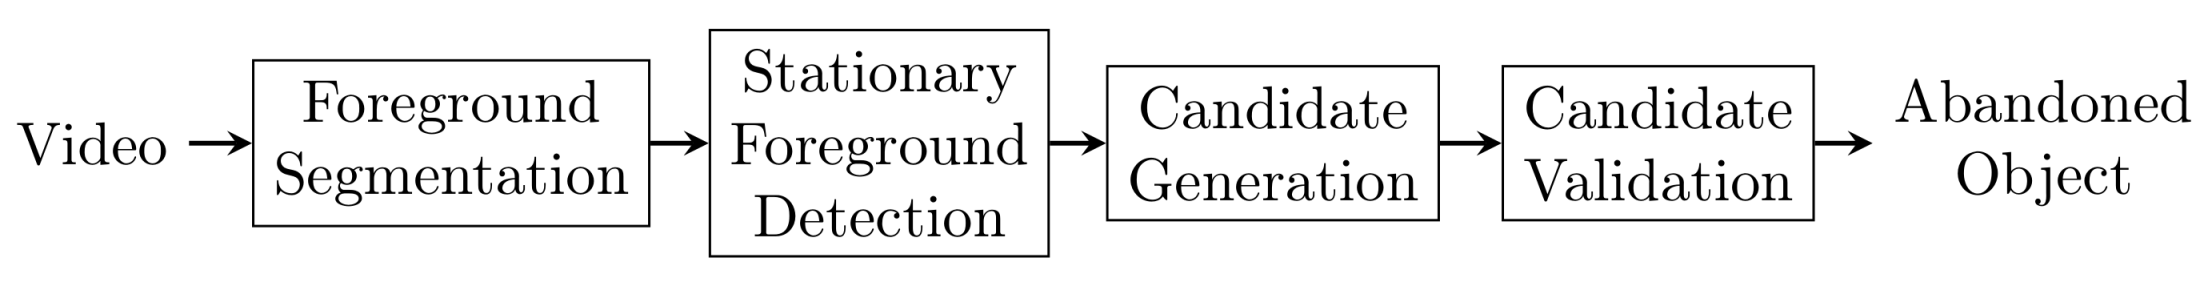
\includegraphics[width=0.85\textwidth]{Images/introduccion/canonical-framework-aod.png}
\caption{\label{fig:canonical-framework-aod}Marco de referencia en detección de objetos abandonados}
\end{figure}

\end{frame}

%%%%%%%%%%%%%%%%%%%%%%%%%%%%%%%%%%%%%%%%%%%%%%%%%%%%%%%%%%%%%%%%%

\begin{frame}{Introducción}

\justifying
En los últimos años se ha mostrado un gran progreso en la detección de personas debido a la aparición de métodos de aprendizaje profundo o \textit{Deep Learning}.

\begin{figure}[ht]
\centering
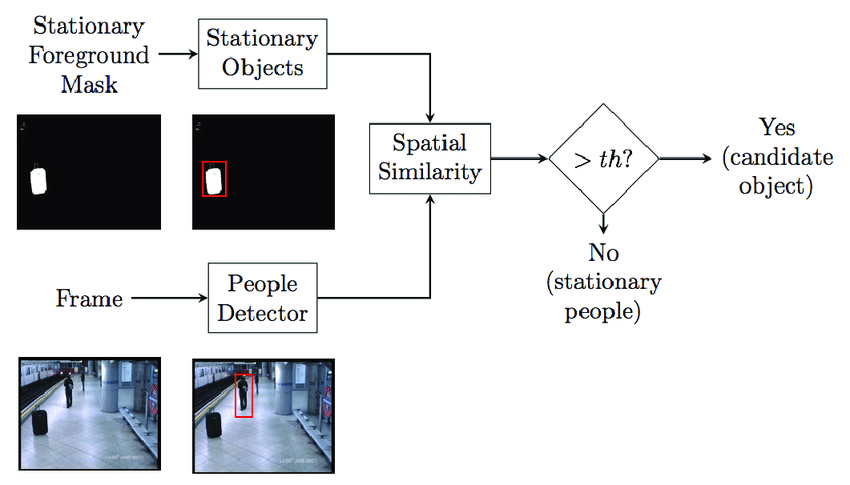
\includegraphics[width=0.65\textwidth]{Images/introduccion/Block-diagram-Stationary-detection.png}
\caption{\label{fig:diagram-stationary-detection}Diagrama de bloques del módulo de generación de candidatos}
\end{figure}
    
\end{frame}

%%%%%%%%%%%%%%%%%%%%%%%%%%%%%%%%%%%%%%%%%%%%%%%%%%%%%%%%%%%%%%%%%

\subsection{Objetivos}

\begin{frame}{Introducción}{Objetivos}

\begin{exampleblock}{Una meta}
\justifying
El objetivo que se persigue es el desarrollo de una estrategia de detección de objetos abandonados mediante el uso de CNN en aplicaciones de videovigilancia en espacios como aeropuertos, estaciones de metro, edificios o cualquier tipo de infraestructura que disponga de una o varias cámaras de videovigilancia.
\end{exampleblock}

\vspace{0.3cm}
Para alcanzar dicho objetivo, se plantearon los siguientes puntos:
\vspace{0.1cm}

\begin{itemize}
    \justifying
    \item Revisión del Estado de Arte.
    \item Evaluación de algoritmos de detección de objetos más relevantes.
    \item Evaluación de algoritmos de seguimiento o de objetos más relevantes.
    \item Implementación y evaluación de un algoritmo de detección de objetos abandonados.
\end{itemize}
  
\end{frame}